\section{Beschreibung der gemessenen Daten}
\subsection{Similarity}
Die Messgröße, die in unserem Experiment gemessen wurde, ist die Similarity $S$.
Diese beschreibt, welcher Anteil der gesendeten Informationen korrekt von Bob
rekonstruiert werden konnte. Dies lässt sich über folgende Relation ausdrücken:
\begin{equation}
S = \frac{N_{\mathrm{korr}}}{N_{\mathrm{ges}}}\,,
\end{equation}
wobei $N_{\mathrm{korr}}$ die Anzahl der Bits im Schlüssel von Bob ist,
die nach der Bereinigung durch ungleiche Basiswahl verbleiben und mit den von
Alice gesendeten Bits übereinstimmen. Die Similarity $S$ wird mit der Gesamtlänge
$N_{\mathrm{ges}}$ des Schlüssels normiert, so dass $S \in [0,1]$ ergibt.

Die Zahl der richtig rekonstruierten Bits hängt hierbei von der Wahl der
Umstände ab, wie zum Beispiel der Kalibration der optischen Linsen und Filter, oder
auch von der Laser-Puls-Frequenz. Um diese Abhängigkeiten zu untersuchen, haben
wir verschiedene Messreihen aufgenommen. Für jeweils eine eingestellte Frequenz
wurde der Dämpfungsexponent der Lichtquelle durch Hinzufügen oder Entfernen eines Filters
bekannter Stärke verändert und anschließend wurde die Similarity bestimmt. Die
zugehörigen Messdaten können in Anhang \ref{sec:messwerttabellen} eingesehen
werden.


\begin{figure*}[htb]
 \centering
%  \includegraphics[page=8,viewport=166 482 445 565,clip,%
%   width=0.8\paperwidth,keepaspectratio]{%
%   ../doc/crypto3}
 \caption{Aufbau des Experiments}
 \label{fig:sim_frequenz}
\end{figure*}

\begin{figure*}[htb]
 \centering
%  \includegraphics[page=8,viewport=166 482 445 565,clip,%
%   width=0.8\paperwidth,keepaspectratio]{%
%   ../doc/crypto3}
 \caption{Aufbau des Experiments}
 \label{fig:sim_alpha}
\end{figure*}

\subsection{Einfluss der Parameter auf die Similarity}

Mit kleiner werdenden Frequenzen nimmt die Similarity unabhängig von der
gewählten Dämpfung ab. Eine Begründung hierfür könnte der Einfluss des
Streulichtes sein. Als mögliche Quellen wäre das verbleibende Umgebungslicht 
im Labor denkbar, danaben aber auch Wärmestrahlung. Thermische Prozesse im
Detektor tragen ebenfalls ein Teil zum Fehler bei.
Wenn man davon ausgeht, dass die Anzahl der Streuphotonen pro
Zeitintervall konstant bleibt, so steigt der relative Fehler und damit auch die
Similarity, wenn im gleichen Zeitfenster nur wenige Photonen des Signals den
Detektor erreichen. Bei hohen Frequenzen dagegen macht der Anteil des
Streulichtes am Gesamtsignal im Detektor nur einen geringen Prozentsatz aus,
wodurch die Similarity größere Werte annimmt.

Es kann davon ausgegangen werden, dass ab einer optimalen Frequenz $f_0(α)$ die
Similarity wieder abnimmt, da die Trägheit/Schaltgeschwindigkeit der EOMs nicht
mehr vernachlässigbar ist oder die Zeitauflösung des Detektors nicht mehr
ausreichend ist. Weiterhin gelangen bei sehr hohen Frequenzen auch die Signallaufzeiten
der elektrischen Anschlüsse an Relevanz.

Auf der anderen Seite überträgt sich auch die Unsicherheit in der Kalibration
der verwendeten Polarisationszustände auch auf die Similarity, die ihrerseits
ebenso ein Ausdruck für die Unsicherheit der Übertragung ist. Sind die
EOMs nicht exakt orthogonal oder parallel ausgerichtet, so ist die
Wahrscheinlichkeit nicht verschwindend, dass ein Photon bei zueinander
orthogonalen/parallelen Zuständen dennoch gemessen/nicht gemessen wird. Dieser
Fehler führt direkt zur Reduzierung der Similarity.

Durch die Wechselwirkung mit Materie kann ein Photon auf dem Weg von Alice zu
Bob ebenfalls seine spezifische Polarisation verlieren. Daher sollte ein Aufheizen,
Einstauben, oder Verschmutzen der Apparatur möglichst ausgeschlossen werden, dies
lässt sich jedoch nur unter größerem Aufwand erreichen.

-weniger Dämpfung -> mehr Photonen -> Bob könnte angreifen (bei uns egal)
                                   -> mehr Streulicht durch Mehrfachreflexion an Geräten
-mehr Dämpfung -> Einfluss von Streulicht wächst, da Signal/Rauschen verhältnis sinkt

-fitten nicht möglich, da zu wenig Messpunkte
-fehler für similarity benötigt weiterer untersuchungen um systematik quantifizieren
zu können
